% ============================================================================
%  Persistent Homology for Parameter-Free Spectral Line Decomposition
%  AASTeX v6.3.1 — ApJ pre-print
% ============================================================================
\documentclass[twocolumn,twocolappendix]{aastex631}

% --- Packages ---------------------------------------------------------------
\usepackage{amsmath,amssymb}
\usepackage{graphicx}
\usepackage{tikz}
\usetikzlibrary{shapes.geometric,arrows.meta,positioning,calc,decorations.pathreplacing}
\usepackage{booktabs}
\usepackage{xcolor}


% --- Macros -----------------------------------------------------------------
\newcommand{\phspectra}{\textsc{PHSpectra}}
\newcommand{\gausspyp}{\textsc{GaussPy+}}
\newcommand{\gausspy}{\textsc{GaussPy}}
\newcommand{\rohsa}{\textsc{ROHSA}}
\newcommand{\srms}{\sigma_{\mathrm{rms}}}
\newcommand{\pmin}{\pi_{\mathrm{min}}}
\newcommand{\aicc}{\mathrm{AICc}}

% --- Metadata ---------------------------------------------------------------
\shorttitle{Persistent Homology for Spectral Line Decomposition}
\shortauthors{Vera-Ciro}

% ============================================================================
\begin{document}

\title{Persistent Homology for Parameter-Free Spectral Line Decomposition}

\author{Carlos Vera-Ciro}
\affiliation{Independent Researcher}

% ---------------------------------------------------------------------------
% ABSTRACT
% ---------------------------------------------------------------------------
\begin{abstract}
Decomposing radio spectral lines into individual Gaussian components is
essential for studying the interstellar medium, yet existing automated methods
require multiple trained parameters.  This work presents \phspectra, a new approach
that uses 0-dimensional persistent homology to detect peaks in 1D spectra.
Persistent homology tracks the birth and death of connected components in the
signal's upper-level sets as a threshold descends from the global maximum,
assigning each peak a topological persistence that measures its significance
without smoothing or differentiation.  The sole free parameter is $\beta$,
which sets the persistence threshold in units of noise:
$\pmin = \beta \cdot \srms$.  On a synthetic benchmark of 350 spectra spanning
seven difficulty categories, \phspectra\ achieves an overall $F_1$ score of 0.925
at the optimal $\beta = 2.8$, with performance varying by only 0.040 across
$\beta \in [2.0, 4.5]$.  Compared with \gausspyp\ on 4200 real ${}^{13}$CO
spectra from the Galactic Ring Survey, \phspectra\ produces lower residual RMS
in 62\% of head-to-head comparisons and runs $2.0\times$ faster, while
requiring no parameter training.  The software is open-source and available at
\url{https://github.com/caverac/phspectra}.
\end{abstract}

\keywords{methods: data analysis --- ISM: kinematics and dynamics ---
          techniques: spectroscopic --- radio lines: ISM}

% ============================================================================
% §1  INTRODUCTION
% ============================================================================
\section{Introduction}\label{sec:intro}

Radio spectral lines --- HI 21\,cm, ${}^{13}$CO, and other molecular
tracers --- encode the kinematic structure of the interstellar medium along
each line of sight.  A single spectrum is typically a superposition of
Gaussian components, each arising from a distinct gas cloud with its own
velocity, velocity dispersion, and column density.  Recovering these
components from a blended spectrum is a blind decomposition problem: one
must determine the number of components~$N_{\mathrm{components}}$ and the three parameters
(amplitude, mean, width) of each without prior knowledge of the true model.
Modern Galactic plane surveys such as the GRS \citep{Jackson2006},
GALFA-HI \citep{Peek2018}, THOR \citep{Beuther2016}, and SEDIGISM
\citep{Schuller2021} produce millions of spectra, making fully automated
decomposition essential.

A variety of automated approaches have been developed, each with distinct
trade-offs.  Derivative spectroscopy methods such as \gausspy\
\citep{Lindner2015} and \gausspyp\ \citep{Riener2019} identify peaks via
smoothed derivatives, but require tuning of smoothing scales $\alpha_1$ and
$\alpha_2$ on synthetic spectra tailored to each survey.  Semi-interactive
toolkits such as \textsc{scousepy} \citep{Henshaw2016Scousepy} and
\textsc{pyspeckit} \citep{Ginsburg2011} enable human-in-the-loop fitting,
but scaling these workflows to millions of spectra is labor-intensive.
Probabilistic component detection methods such as \textsc{PySpecNest}
\citep{Sokolov2020} provide rigorous uncertainty quantification at the cost
of high per-spectrum computation.  GPU-accelerated fitters such as
\textsc{SPIF} \citep{Colombo2024} and survey-specific pipelines
(e.g., \textsc{mwydyn}; \citealt{Rigby2024}) target high throughput but rely
on specialized implementations.  Deep reinforcement learning
(\textsc{Spectuner-D1}; \citealt{Li2025}) learns a decomposition policy from
labeled training spectra.
Regularized optimization (\rohsa; \citealt{Marchal2019}) enforces spatial
coherence in data cubes but introduces regularization weights that must be
tuned.  The common thread is that existing methods require multiple
parameters or training choices that depend on the data.

This paper presents \phspectra, a new approach that uses
0-dimensional persistent homology for peak detection in spectral-line
decomposition
\citep{Edelsbrunner2002,Zomorodian2005}.  Topological data analysis (TDA)
remains relatively niche in astronomy, with representative examples in
cosmic-web topology \citep{Xu2019} and cosmic-shear statistics
\citep{Heydenreich2022}; closely related structure-finding tools such as
\textsc{SUBFIND} \citep{Springel2001} have long been standard in simulations.
To the best of my knowledge, this is the first application
of persistent homology to spectral line decomposition.  The algorithm has a
single free parameter~$\beta$ (the persistence threshold in units of noise),
requires no expensive training, and runs in $O(n \log n)$ time.  It is shown that it
achieves high accuracy on synthetic data while matching or exceeding
\gausspyp\ on real GRS spectra without training.  The method is presented in
\S\ref{sec:method}, evaluate it on synthetic and real ${}^{13}$CO spectra in
\S\ref{sec:evaluation}, examine $\beta$ sensitivity in
\S\ref{sec:beta}, compare performance in \S\ref{sec:performance}, discuss
limitations and context in \S\ref{sec:discussion}, and summarize the
conclusions in \S\ref{sec:summary}.

% ============================================================================
% §2  METHOD
% ============================================================================
\section{Method}\label{sec:method}


\begin{figure*}[t!]
  \centering
  \includegraphics[width=0.9\textwidth]{figures/img/water-level-stages.png}
  \caption{%
    The descending water-level interpretation of 0-dimensional persistent
    homology, applied to a synthetic three-peak spectrum.  As the threshold
    $t$ (dashed line) decreases, connected components are born at local maxima
    and die when they merge into an older component.  Red dots mark peak births;
    annotations show the final persistence $\pi = b - d$.  \emph{Top left}:
    $t$ above all peaks (empty upper-level set).  \emph{Top right}: peak~A
    ($\pi = 2.58$) is born as the global maximum.  \emph{Bottom left}: peak~B
    ($\pi = 1.20$) appears as a second island.  \emph{Bottom right}: peak~C
    ($\pi = 0.73$) dies when its island merges with~A's.
    \label{fig:waterlevel}}
\end{figure*}

The \phspectra\ algorithm is described in four stages: peak detection via
persistent homology (\S\ref{sec:persistence}), conversion of topological peaks
to Gaussian candidates (\S\ref{sec:candidates}), nonlinear least-squares
fitting (\S\ref{sec:fitting}), and iterative refinement guided by the
corrected Akaike Information Criterion (\S\ref{sec:refinement}).

% ---------------------------------------------------------------------------
% §2.1  Persistent homology for 1D peak detection
% ---------------------------------------------------------------------------
\subsection{Persistent homology for 1D peak detection}\label{sec:persistence}

Given a discrete 1D signal $f : \{0, 1, \ldots, n{-}1\} \to \mathbb{R}$, the method
defines the \emph{upper-level set} at threshold $t$ as
\begin{equation}
  U_t = \bigl\{\, i \;\big|\; f(i) \geq t \,\bigr\}.
\end{equation}
As $t$ decreases from $\max(f)$ toward $-\infty$, the topology of $U_t$
changes: new connected components are \emph{born} when $t$ drops below a
local maximum, and two components \emph{merge} when their supporting
intervals connect.  At each merger, the younger component --- the one whose
maximum is lower --- \emph{dies} at the current threshold.  This is
0-dimensional persistent homology ($H_0$): tracking connected components
across a filtration parameterized by $t$
\citep{Edelsbrunner2002,Edelsbrunner2008}.

Each local maximum (except the global one) produces a birth--death pair
$(b, d)$ where $b = f(i)$ is the peak height, $d$ is the merge threshold,
and the \emph{persistence}
\begin{equation}\label{eq:persistence}
  \pi = b - d
\end{equation}
quantifies how prominent the peak is.  The global maximum never merges; it
has $d = 0$ and persistence equal to its height.  Persistence provides a
scale-independent ranking of peaks: high-persistence features correspond to
real signal; low-persistence features are noise fluctuations.  No smoothing
or differentiation is required.
Implementation is straightforward: samples are processed in order of
decreasing function value, and a union-find data structure tracks connected
components.  When a newly visited index has an already-visited neighbor
belonging to a different component, the two components are merged and the
younger one's death is recorded.  Sorting the $n$ samples costs
$O(n \log n)$; each union-find operation is amortized $O(\alpha(n))$, where
$\alpha$ is the inverse Ackermann function, so the total complexity is
dominated by the initial sort.

Raw persistence is measured in the same units as the signal, so a fixed
threshold cannot distinguish noise from signal across datasets with different
noise levels.  The minimum persistence is therefore set in units of the
noise:
\begin{equation}\label{eq:threshold}
  \pmin = \beta \cdot \srms,
\end{equation}
where $\srms$ is the noise RMS estimated from the data (see
\S\ref{sec:candidates}) and $\beta$ is the sole free parameter of the model.
The default value $\beta = 3.5$ corresponds to a $3.5\sigma$ persistence cut.\\

The name of this approach (Persistent Homology) reflects two ideas.  \emph{Homology} refers to the
algebraic-topological invariants that count features of different
dimensions: connected components ($H_0$), loops ($H_1$), voids ($H_2$),
and so on \citep{Zomorodian2005}.  For 1D peak detection only $H_0$ is
needed: each connected component of the upper-level set corresponds to a
peak.  \emph{Persistent} means that these invariants are tracked across the
full filtration parameterized by~$t$, not evaluated at a single threshold.
The lifetime of each component --- its persistence --- provides a
parameter-free ranking of feature significance that is stable under
perturbation \citep{Edelsbrunner2002,Otter2017}.  The union-find data
structure \citep{Tarjan1975} makes the computation efficient.

This suits spectral decomposition because most methods must commit early to
either a model family, a smoothing scale, or a heuristic for deciding which
peaks are worth fitting, all of which can bias the decomposition when lines
are blended or span a wide range of widths.  Persistent homology avoids a
single-scale commitment by descending through all thresholds, detecting peaks
at every scale simultaneously and ranking them by a single intrinsic measure
--- persistence --- that is directly comparable across features of different
amplitudes and widths.  A faint broad component and a bright narrow component
are treated on equal footing; no special tuning is required to accommodate
both.

Figure~\ref{fig:waterlevel} uses the descending water-level interpretation on
a synthetic three-peak spectrum.  As the water level (threshold) drops past
each local maximum, a new connected component (``island'') is born; when two
islands merge, the younger one dies and its persistence is recorded.  The
three real peaks have persistence values of $\pi = 2.58$, $1.20$, and $0.73$
--- well separated from the near-zero persistence of noise fluctuations.  In
practice these values are compared against the minimum persistence
$\pmin = \beta\,\srms$: peaks with $\pi > \pmin$ are kept as Gaussian
candidates, while lower-persistence features are rejected as noise.


The same information can be represented in a persistence diagram
\citep{Edelsbrunner2002,Edelsbrunner2008}, where each peak is a point $(b, d)$
above the diagonal $b = d$; high-persistence peaks sit well away from the
diagonal, and a horizontal cut at $\pmin$ separates signal from noise.

% ---------------------------------------------------------------------------
% §2.2  From persistence to Gaussian candidates
% ---------------------------------------------------------------------------
\subsection{From persistence to Gaussian candidates}\label{sec:candidates}

Before peak detection, \phspectra\ estimates $\srms$ using a signal-masked
approach following \citet{Riener2019}, Section~3.1.1.  Runs of more than two
consecutive positive channels are masked (with two-channel padding on each
side) to exclude spectral features.  The median absolute deviation (MAD) of
the remaining negative channels provides an initial robust scale estimate.
Channels exceeding $\pm 5\,\sigma_{\mathrm{MAD}}$ are then clipped, and the
final RMS is computed as $\srms^2 = \sum_i f_i^2/N_{\mathrm{sur}}$, where the sum
runs over the $N_{\mathrm{sur}}$ surviving channels.  This procedure avoids biasing the noise estimate with
real emission and provides the noise scale used to set the persistence
threshold $\pmin = \beta \cdot \srms$.

Each peak surviving this threshold becomes an initial Gaussian guess.  The
amplitude is taken directly from the peak height, $a_0 = f(\mathrm{index})$,
and the mean is the peak channel index.  For non-global peaks, the initial
width is estimated from the persistence birth--death pair,
\begin{equation}\label{eq:sigma0}
  \sigma_0 = \frac{d}{\sqrt{2\ln(b / d_v)}},
\end{equation}
where $b$ is the peak birth value, $d_v$ the death value (the threshold at
which the peak merges with a higher component), and $d$ is the channel
distance between the peak and the merge point.  For the global maximum (which
has no death event), $\sigma_0 = 1.0$ channel is used as a fallback.  Peaks
are ordered by persistence (most significant first).  When the number of
candidates exceeds the internal parameter limit of the least-squares solver,
they are fitted in batches: the most persistent peaks are fitted against the
full signal first, then remaining peaks are fitted against the residual, and
all surviving components are combined into a single joint refit.

% ---------------------------------------------------------------------------
% §2.3  Gaussian fitting
% ---------------------------------------------------------------------------
\subsection{Gaussian fitting}\label{sec:fitting}

The initial guesses are fitted simultaneously as a sum of $K$ (the number of peaks
that survive the persistence threshold) Gaussians:
\begin{equation}\label{eq:model}
  F(x) = \sum_{i=1}^{K} a_i \exp\!\left(-\frac{(x - \mu_i)^2}{2\sigma_i^2}\right),
\end{equation}
using bounded nonlinear least-squares optimization.  The primary solver is a
custom C extension implementing the Levenberg--Marquardt algorithm with
analytic Jacobians, which provides the tight per-call overhead needed for
survey-scale processing.  If the C extension is unavailable (e.g.\ in a
pure-Python installation), \phspectra\ falls back to
\texttt{scipy.optimize.curve\_fit} \citep{Virtanen2020}.  In both cases the
bounds enforce $a_i \geq 0$, $\mu_i \in [0, n)$, and
$\sigma_i \in [0.3, n/2]$ channels.  Because the persistence-detected peak
positions and amplitudes are already close to the true values, the optimizer
typically converges in few iterations --- its primary task is to determine
the correct widths and fine-tune positions and amplitudes.

% ---------------------------------------------------------------------------
% §2.4  Iterative refinement
% ---------------------------------------------------------------------------
\subsection{Iterative refinement}\label{sec:refinement}

After the initial fit, components are validated once: a component is
rejected if any of the following hold: (a)~FWHM $< 1$ channel; (b)~mean
outside the spectrum; (c)~amplitude $< 1.5\,\srms$ (SNR floor); or
(d)~matched-filter signal-to-noise ratio $< 5.0$, where the matched-filter
SNR of component~$i$ is defined as
\begin{equation}\label{eq:snr_mf}
  \mathrm{SNR}_{\mathrm{mf},i} = \frac{a_i}{\srms}\,
    \sqrt{\sigma_i}\;\pi^{1/4}.
\end{equation}
This quantity measures the detectability of a Gaussian component of
amplitude~$a_i$ and width~$\sigma_i$ against noise of level~$\srms$.
If any components are rejected, the remaining ones are refit.

The validated model is then scored using the corrected Akaike Information
Criterion \citep{Akaike1974,Hurvich1989}:
\begin{equation}\label{eq:aicc}
  \aicc = N \ln\!\left(\frac{\mathrm{RSS}}{N}\right) + 2k
        + \frac{2k^2 + 2k}{N - k - 1},
\end{equation}
where $\mathrm{RSS} = \sum_j (f_j - F_j)^2$ is the residual sum of squares,
$k = 3K$ is the number of free parameters (three per Gaussian component),
and $N$ is the number of spectral channels.  If no residual peaks or blended
pairs are found, the result is returned without further refinement.

Otherwise, the model enters an iterative refinement loop of up to three
iterations.  Each iteration performs three operations:

\begin{enumerate}
  \item \textbf{Residual peak search.}  The persistence detection algorithm is
    run on the residual spectrum (data minus model) with a lower threshold of
    $1.5\,\srms$ to find missed components.  Any peaks found are validated and
    added to the model.

  \item \textbf{Negative dip splitting.}  If the residual contains a dip
    exceeding $-5\,\srms$, the broadest Gaussian component overlapping that
    channel is split into two narrower components.

  \item \textbf{Blended pair merging.}  If two components are separated by
    less than $1.2 \times \min(\mathrm{FWHM}_i, \mathrm{FWHM}_j)$, they are
    merged into a single flux-weighted component.
\end{enumerate}

After each operation, the full model is refit via least-squares, and the
modification is accepted only if $\aicc$ decreases.  The loop terminates when
no operation produces an improvement or the iteration limit is reached.

Figure~\ref{fig:pipeline} summarizes the complete pipeline from raw spectrum
to final Gaussian components.

\begin{figure}[t!]
  \centering
  \resizebox{\columnwidth}{!}{% Pipeline overview flowchart for phspectra
% Included via % Pipeline overview flowchart for phspectra
% Included via % Pipeline overview flowchart for phspectra
% Included via \input{figures/tikz/pipeline-overview.tex} in ms.tex
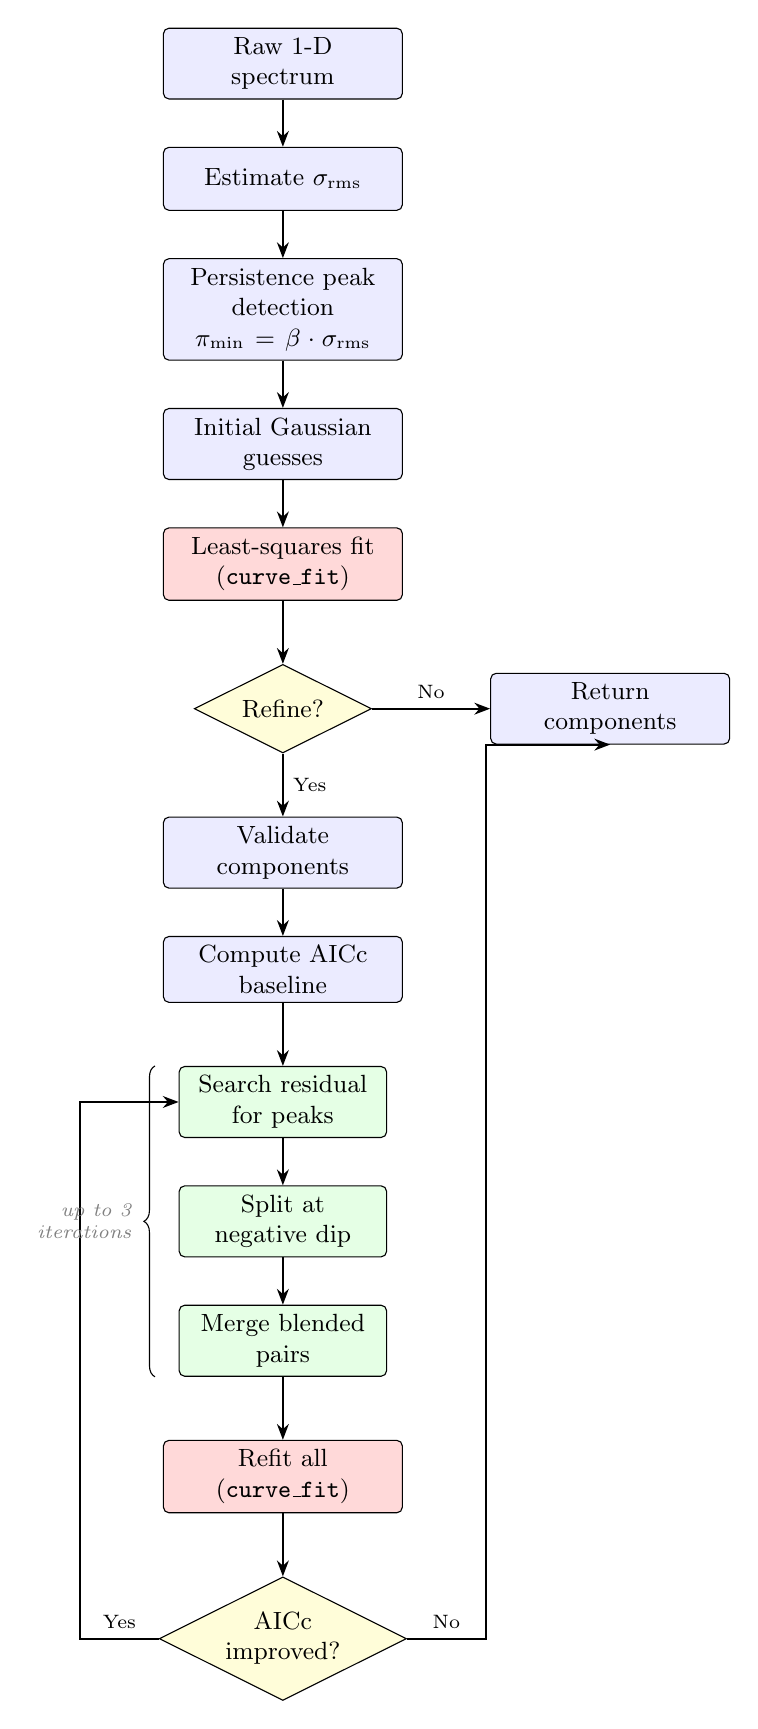
\begin{tikzpicture}[
    node distance=6mm and 4mm,
    every node/.style={font=\small},
    block/.style={
      rectangle, draw, rounded corners=2pt,
      text width=28mm, minimum height=8mm,
      align=center, fill=blue!8
    },
    decision/.style={
      diamond, draw, aspect=2,
      text width=16mm, align=center,
      inner sep=1pt, fill=yellow!15
    },
    fitblock/.style={
      rectangle, draw, rounded corners=2pt,
      text width=28mm, minimum height=8mm,
      align=center, fill=red!15
    },
    refineblock/.style={
      rectangle, draw, rounded corners=2pt,
      text width=24mm, minimum height=7mm,
      align=center, fill=green!10
    },
    arr/.style={-{Stealth[length=2mm]}, thick},
    note/.style={font=\scriptsize\itshape, text=gray}
  ]

  % Main pipeline
  \node[block] (input) {Raw 1-D\\spectrum};
  \node[block, below=of input] (rms) {Estimate $\srms$};
  \node[block, below=of rms] (persist) {Persistence peak\\detection\\$\pmin = \beta \cdot \srms$};
  \node[block, below=of persist] (guess) {Initial Gaussian\\guesses};
  \node[fitblock, below=of guess] (fit) {Least-squares fit\\(\texttt{curve\_fit})};
  \node[decision, below=8mm of fit] (refineq) {Refine?};

  % No-refine path
  \node[block, right=15mm of refineq] (output) {Return\\components};

  % Refine path
  \node[block, below=8mm of refineq] (validate) {Validate\\components};
  \node[block, below=of validate] (aiccbase) {Compute AICc\\baseline};

  % Refinement loop
  \node[refineblock, below=8mm of aiccbase] (residual) {Search residual\\for peaks};
  \node[refineblock, below=of residual] (split) {Split at\\negative dip};
  \node[refineblock, below=of split] (merge) {Merge blended\\pairs};
  \node[fitblock, below=8mm of merge] (refit) {Refit all\\(\texttt{curve\_fit})};
  \node[decision, below=8mm of refit] (improved) {AICc\\improved?};

  % Arrows — main path
  \draw[arr] (input) -- (rms);
  \draw[arr] (rms) -- (persist);
  \draw[arr] (persist) -- (guess);
  \draw[arr] (guess) -- (fit);
  \draw[arr] (fit) -- (refineq);
  \draw[arr] (refineq) -- node[above] {\scriptsize No} (output);
  \draw[arr] (refineq) -- node[right] {\scriptsize Yes} (validate);
  \draw[arr] (validate) -- (aiccbase);
  \draw[arr] (aiccbase) -- (residual);
  \draw[arr] (residual) -- (split);
  \draw[arr] (split) -- (merge);
  \draw[arr] (merge) -- (refit);
  \draw[arr] (refit) -- (improved);

  % Accept → loop back
  \draw[arr] (improved.west) -- ++(-10mm,0)
    node[above, pos=0.5] {\scriptsize Yes}
    |- (residual.west);

  % Reject → output
  \draw[arr] (improved.east) -- ++(10mm,0)
    node[above, pos=0.5] {\scriptsize No}
    |- (output.south);

  % Brace for refinement loop
  \draw[decorate, decoration={brace, amplitude=4pt, mirror}]
    ([xshift=-3mm]residual.north west) -- ([xshift=-3mm]merge.south west)
    node[midway, left=5pt, note, text width=12mm, align=right]
    {up to 3\\iterations};

\end{tikzpicture}
 in ms.tex
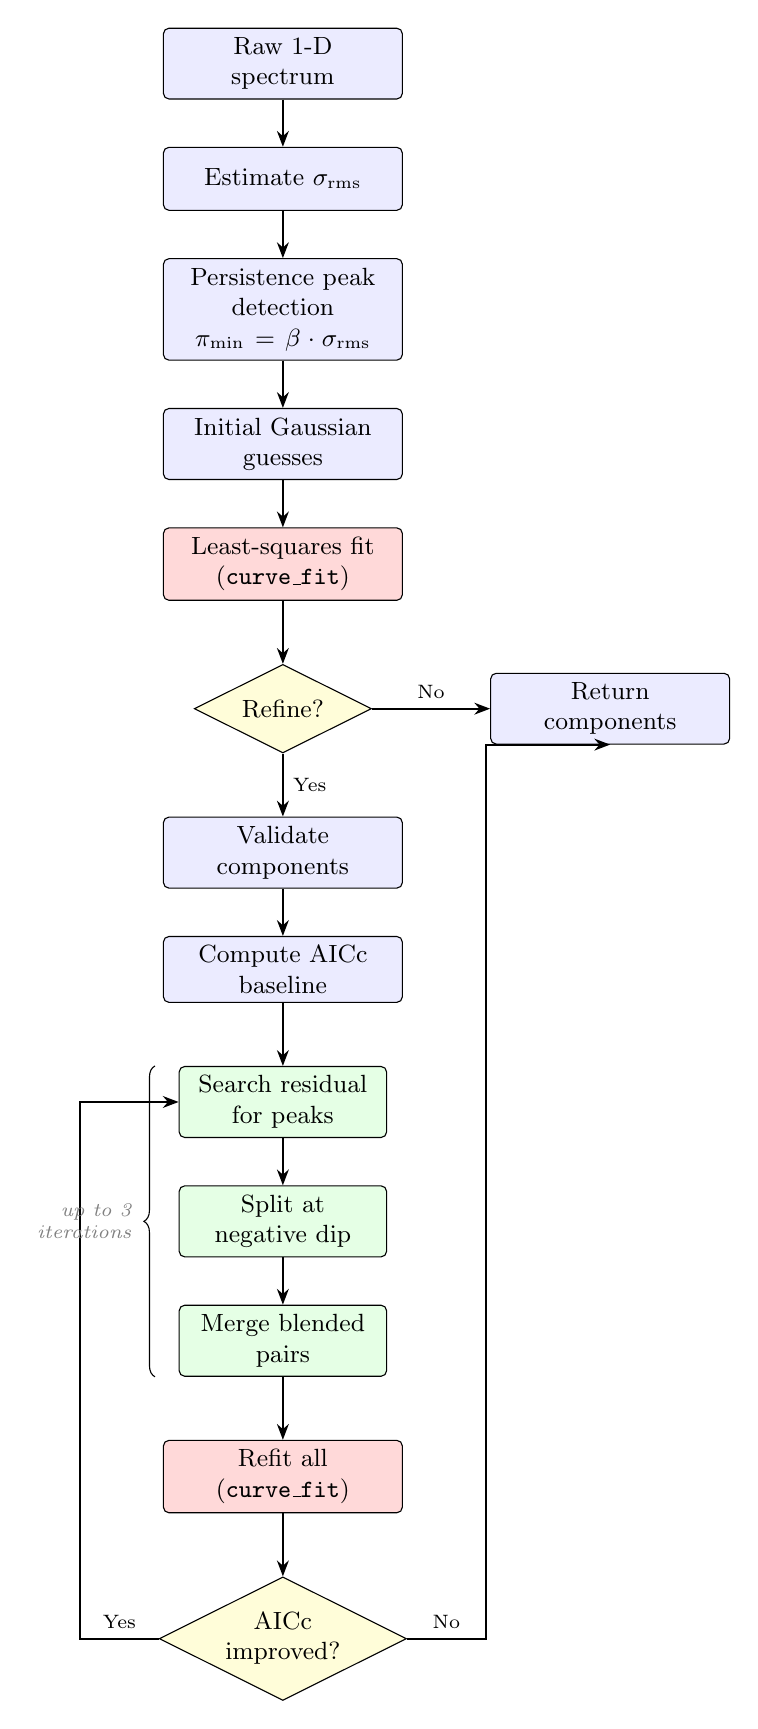
\begin{tikzpicture}[
    node distance=6mm and 4mm,
    every node/.style={font=\small},
    block/.style={
      rectangle, draw, rounded corners=2pt,
      text width=28mm, minimum height=8mm,
      align=center, fill=blue!8
    },
    decision/.style={
      diamond, draw, aspect=2,
      text width=16mm, align=center,
      inner sep=1pt, fill=yellow!15
    },
    fitblock/.style={
      rectangle, draw, rounded corners=2pt,
      text width=28mm, minimum height=8mm,
      align=center, fill=red!15
    },
    refineblock/.style={
      rectangle, draw, rounded corners=2pt,
      text width=24mm, minimum height=7mm,
      align=center, fill=green!10
    },
    arr/.style={-{Stealth[length=2mm]}, thick},
    note/.style={font=\scriptsize\itshape, text=gray}
  ]

  % Main pipeline
  \node[block] (input) {Raw 1-D\\spectrum};
  \node[block, below=of input] (rms) {Estimate $\srms$};
  \node[block, below=of rms] (persist) {Persistence peak\\detection\\$\pmin = \beta \cdot \srms$};
  \node[block, below=of persist] (guess) {Initial Gaussian\\guesses};
  \node[fitblock, below=of guess] (fit) {Least-squares fit\\(\texttt{curve\_fit})};
  \node[decision, below=8mm of fit] (refineq) {Refine?};

  % No-refine path
  \node[block, right=15mm of refineq] (output) {Return\\components};

  % Refine path
  \node[block, below=8mm of refineq] (validate) {Validate\\components};
  \node[block, below=of validate] (aiccbase) {Compute AICc\\baseline};

  % Refinement loop
  \node[refineblock, below=8mm of aiccbase] (residual) {Search residual\\for peaks};
  \node[refineblock, below=of residual] (split) {Split at\\negative dip};
  \node[refineblock, below=of split] (merge) {Merge blended\\pairs};
  \node[fitblock, below=8mm of merge] (refit) {Refit all\\(\texttt{curve\_fit})};
  \node[decision, below=8mm of refit] (improved) {AICc\\improved?};

  % Arrows — main path
  \draw[arr] (input) -- (rms);
  \draw[arr] (rms) -- (persist);
  \draw[arr] (persist) -- (guess);
  \draw[arr] (guess) -- (fit);
  \draw[arr] (fit) -- (refineq);
  \draw[arr] (refineq) -- node[above] {\scriptsize No} (output);
  \draw[arr] (refineq) -- node[right] {\scriptsize Yes} (validate);
  \draw[arr] (validate) -- (aiccbase);
  \draw[arr] (aiccbase) -- (residual);
  \draw[arr] (residual) -- (split);
  \draw[arr] (split) -- (merge);
  \draw[arr] (merge) -- (refit);
  \draw[arr] (refit) -- (improved);

  % Accept → loop back
  \draw[arr] (improved.west) -- ++(-10mm,0)
    node[above, pos=0.5] {\scriptsize Yes}
    |- (residual.west);

  % Reject → output
  \draw[arr] (improved.east) -- ++(10mm,0)
    node[above, pos=0.5] {\scriptsize No}
    |- (output.south);

  % Brace for refinement loop
  \draw[decorate, decoration={brace, amplitude=4pt, mirror}]
    ([xshift=-3mm]residual.north west) -- ([xshift=-3mm]merge.south west)
    node[midway, left=5pt, note, text width=12mm, align=right]
    {up to 3\\iterations};

\end{tikzpicture}
 in ms.tex
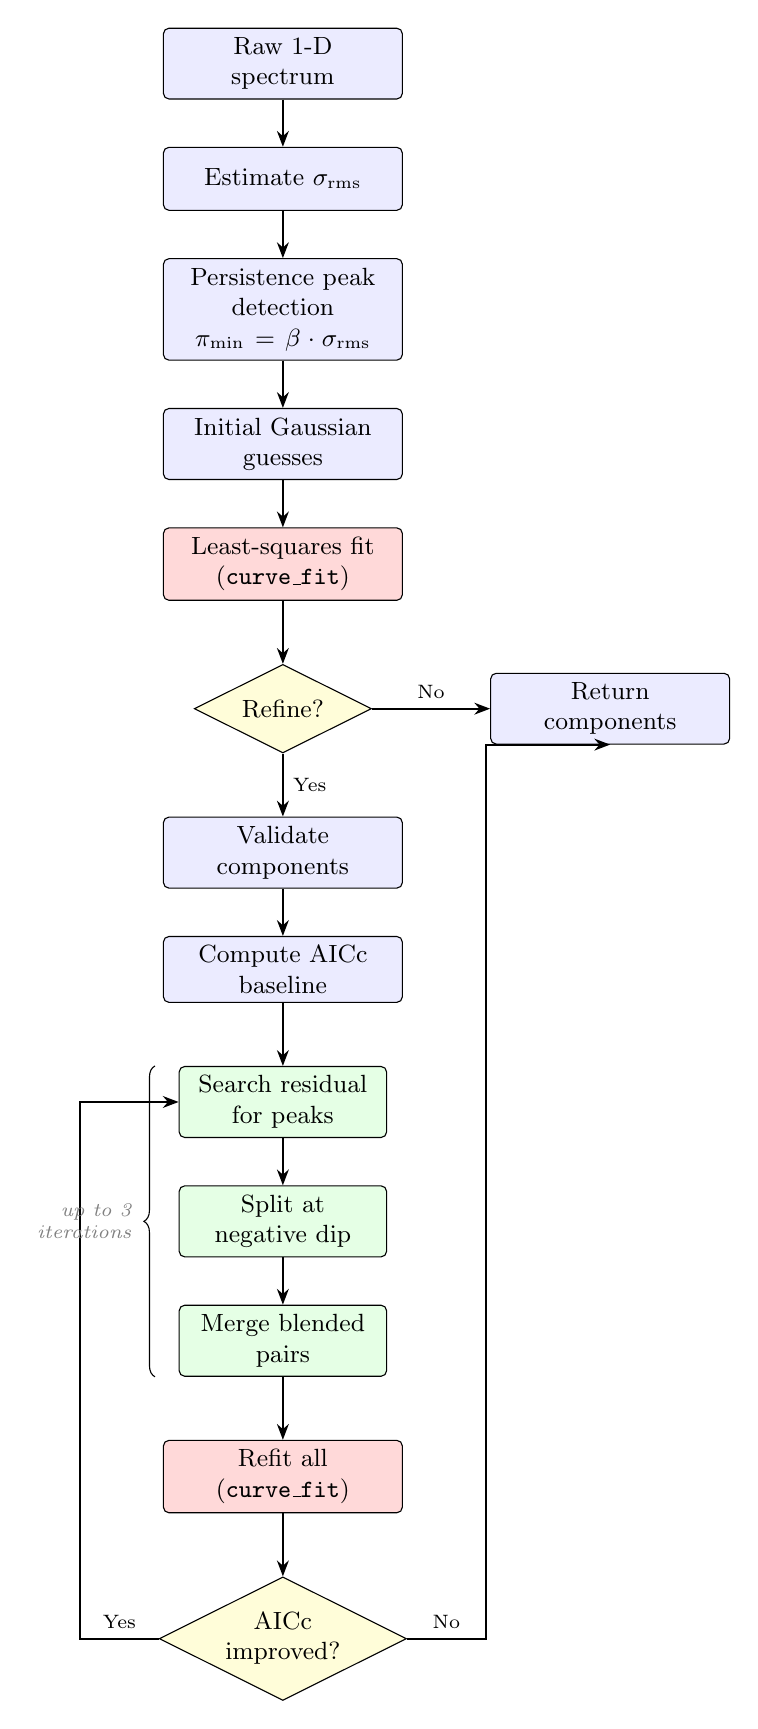
\begin{tikzpicture}[
    node distance=6mm and 4mm,
    every node/.style={font=\small},
    block/.style={
      rectangle, draw, rounded corners=2pt,
      text width=28mm, minimum height=8mm,
      align=center, fill=blue!8
    },
    decision/.style={
      diamond, draw, aspect=2,
      text width=16mm, align=center,
      inner sep=1pt, fill=yellow!15
    },
    fitblock/.style={
      rectangle, draw, rounded corners=2pt,
      text width=28mm, minimum height=8mm,
      align=center, fill=red!15
    },
    refineblock/.style={
      rectangle, draw, rounded corners=2pt,
      text width=24mm, minimum height=7mm,
      align=center, fill=green!10
    },
    arr/.style={-{Stealth[length=2mm]}, thick},
    note/.style={font=\scriptsize\itshape, text=gray}
  ]

  % Main pipeline
  \node[block] (input) {Raw 1-D\\spectrum};
  \node[block, below=of input] (rms) {Estimate $\srms$};
  \node[block, below=of rms] (persist) {Persistence peak\\detection\\$\pmin = \beta \cdot \srms$};
  \node[block, below=of persist] (guess) {Initial Gaussian\\guesses};
  \node[fitblock, below=of guess] (fit) {Least-squares fit\\(\texttt{curve\_fit})};
  \node[decision, below=8mm of fit] (refineq) {Refine?};

  % No-refine path
  \node[block, right=15mm of refineq] (output) {Return\\components};

  % Refine path
  \node[block, below=8mm of refineq] (validate) {Validate\\components};
  \node[block, below=of validate] (aiccbase) {Compute AICc\\baseline};

  % Refinement loop
  \node[refineblock, below=8mm of aiccbase] (residual) {Search residual\\for peaks};
  \node[refineblock, below=of residual] (split) {Split at\\negative dip};
  \node[refineblock, below=of split] (merge) {Merge blended\\pairs};
  \node[fitblock, below=8mm of merge] (refit) {Refit all\\(\texttt{curve\_fit})};
  \node[decision, below=8mm of refit] (improved) {AICc\\improved?};

  % Arrows — main path
  \draw[arr] (input) -- (rms);
  \draw[arr] (rms) -- (persist);
  \draw[arr] (persist) -- (guess);
  \draw[arr] (guess) -- (fit);
  \draw[arr] (fit) -- (refineq);
  \draw[arr] (refineq) -- node[above] {\scriptsize No} (output);
  \draw[arr] (refineq) -- node[right] {\scriptsize Yes} (validate);
  \draw[arr] (validate) -- (aiccbase);
  \draw[arr] (aiccbase) -- (residual);
  \draw[arr] (residual) -- (split);
  \draw[arr] (split) -- (merge);
  \draw[arr] (merge) -- (refit);
  \draw[arr] (refit) -- (improved);

  % Accept → loop back
  \draw[arr] (improved.west) -- ++(-10mm,0)
    node[above, pos=0.5] {\scriptsize Yes}
    |- (residual.west);

  % Reject → output
  \draw[arr] (improved.east) -- ++(10mm,0)
    node[above, pos=0.5] {\scriptsize No}
    |- (output.south);

  % Brace for refinement loop
  \draw[decorate, decoration={brace, amplitude=4pt, mirror}]
    ([xshift=-3mm]residual.north west) -- ([xshift=-3mm]merge.south west)
    node[midway, left=5pt, note, text width=12mm, align=right]
    {up to 3\\iterations};

\end{tikzpicture}
}
  \caption{%
    Flowchart of the \phspectra\ pipeline.  After noise estimation and
    persistence-based peak detection, the initial Gaussian fit is validated
    and scored by AICc.  If residual peaks or blended pairs remain, an
    iterative refinement loop searches for missed components, splits
    over-broad fits at negative residual dips, and merges redundant pairs;
    each modification is accepted only if it lowers the AICc.
    \label{fig:pipeline}}
\end{figure}


% ============================================================================
% §3  EVALUATION
% ============================================================================
\section{Evaluation}\label{sec:evaluation}

\begin{figure}[t!]
  \centering
  \includegraphics[width=\columnwidth]{figures/img/synthetic-f1.png}
  \caption{%
    $F_1$ score versus $\beta$ for each synthetic benchmark category (colored
    lines) and overall (black).  Performance is remarkably stable: the overall
    $F_1$ varies by only 0.040 across $\beta \in [2.0, 4.5]$.
    \label{fig:synthetic_f1}}
\end{figure}


\phspectra\ is evaluated on both synthetic spectra with known ground-truth
components (\S\ref{sec:synthetic}) and real ${}^{13}$CO data from the Galactic
Ring Survey (\S\ref{sec:grs}).

\begin{deluxetable*}{llccclc}
\tablecaption{Synthetic benchmark categories.  Each category contains 50
spectra with the listed parameter ranges and constraints.  All spectra have
424 channels and noise $\sigma = 0.25$~K.  The last column gives the $F_1$
score at the optimal $\beta$.\label{tab:categories}}
\tablehead{
  \colhead{Category} & \colhead{Label} & \colhead{$N_{\mathrm{comp}}$} &
  \colhead{$a$ (K)} & \colhead{$\sigma$ (ch)} & \colhead{Constraint} &
  \colhead{$F_1$}
}
\startdata
Single Bright    & SB  & 1   & 1.0--5.0  & 3--10  & SNR $> 7$                & 0.962 \\
Single Faint     & SF  & 1   & 0.3--0.8  & 3--10  & SNR $2$--$6$             & 0.907 \\
Single Narrow    & SN  & 1   & 1.0--5.0  & 1--2.5 & Sub-resolution           & 0.943 \\
Single Broad     & SBd & 1   & 0.5--3.0  & 10--20 & Extended features        & 0.952 \\
Multi Separated  & MS  & 2--3 & 0.5--4.0 & 2--8   & Sep.\ $> 4\sigma$       & 0.975 \\
Multi Blended    & MB  & 2--3 & 0.5--4.0 & 3--8   & Sep.\ $1.5$--$3\sigma$  & 0.820 \\
Crowded          & C   & 4--5 & 0.3--3.0 & 2--6   & Mixed separations        & 0.936 \\
\enddata
\end{deluxetable*}

% ---------------------------------------------------------------------------
% §3.1  Synthetic benchmark
% ---------------------------------------------------------------------------
\subsection{Synthetic benchmark}\label{sec:synthetic}

A benchmark of 350 synthetic spectra ($50$ per category) was constructed to
span seven categories of increasing difficulty (Table~\ref{tab:categories}).
Each spectrum has 424 channels with additive Gaussian noise at
$\sigma = 0.25$~K, matching the properties of the GRS \citep{Jackson2006}.
Because the true Gaussian components are known exactly, the $F_1$ score measures
true accuracy rather than agreement with another algorithm.  Component
matching uses the Hungarian algorithm with the criteria of
\citet{Lindner2015}: a predicted component matches a true component if the
amplitude ratio is within $[0.5, 2.0]$, the position difference is less than
the larger of the two widths, and the width ratio is within $[0.5, 2.0]$.
$F_1$ is computed as the harmonic mean of precision (fraction of predicted
components that match a true one) and recall (fraction of true components that
are matched).

Figure~\ref{fig:synthetic_f1} shows the $F_1$ score as a function of $\beta$ for
each category and overall measurement.  The overall $F_1$ varies by only 0.040 across the
full sweep from $\beta = 2.0$ to $\beta = 4.5$, confirming the low
sensitivity of the algorithm to this parameter.  At the optimal
$\beta = 2.8$, the overall $F_1$ is 0.925.  The difficulty gradient follows
physical expectations: well-separated multi-component spectra (MS) are
easiest ($F_1$~$= 0.975$), while heavily blended multi-component spectra (MB) are
the most challenging ($F_1$~$= 0.820$), a regime where any algorithm faces
fundamental ambiguity due to overlapping components.  Per-category $F_1$
scores are listed in the last column of Table~\ref{tab:categories}.


Across the $\beta$ sweep, position errors are typically sub-channel, and
amplitude and width relative errors remain small and stable.  These trends
hold across all seven categories.\\

Against real training data the behavior is similar, $F_1$ is highly insensitive
to $\beta$ accross a wide range, with an optimal value at around $\approx 3$.
The practical reason for preferring $\beta=3.5$ is speed. A lower $\beta$ admits
more candidate peaks from the persistence filtration, many of which sit just
above the noise floor. These marginal peaks generate initial Gaussian guesses
that must be fitted by the Levenberg-Marquardt solver -- the most expensive 
step in the pipeline -- only to be discarded during component validation 
(SNR floor, matched-filter SNR). The fitting cost scales with the number of
components, so a large number of doomed candidates slows the algorithm without
improving the final decomposition.\\

At $\beta = 3.5$, the persistence threshold is high enough that most noise 
peaks are rejected before fitting, while genuine features are retained. 
This provides a good balance between not missing real peaks near the detection 
limit and not wasting computation on candidates that will be removed downstream.

% ---------------------------------------------------------------------------
% §3.2  GRS comparison with GaussPy+
% ---------------------------------------------------------------------------
\subsection{GRS comparison with GaussPy+}\label{sec:grs}

\phspectra\ and \gausspyp\ are compared on all 4200 spectra in a GRS test field
from the Galactic Ring Survey \citep[GRS;][]{Jackson2006}, a ${}^{13}$CO
$J = 1 \to 0$ survey of the inner Galaxy.  Each spectrum has 424 velocity
channels.  \gausspyp\ runs with the trained parameters from
\citet{Riener2019}: $\alpha_1 = 2.89$, $\alpha_2 = 6.65$ (two-phase
decomposition), and an SNR threshold of 3.0.  \phspectra\ uses the default
$\beta = 3.5$.

\subsubsection{Residual RMS}\label{sec:rms}

Table~\ref{tab:rms} summarizes the fit quality.  Both tools achieve nearly
identical mean RMS values.  In head-to-head comparisons, \phspectra\ achieves
lower residual RMS on 62\% of spectra (2592 of 4200).  The slightly lower
mean RMS of \gausspyp\ is driven by a tail of spectra where it fits many
more components, reducing RMS at the cost of potential overfitting (see
below).

\begin{deluxetable}{lcc}
\tablecaption{Residual RMS comparison on 4200 GRS spectra.\label{tab:rms}}
\tablehead{
  \colhead{Metric} & \colhead{\phspectra} & \colhead{\gausspyp}
}
\startdata
Mean RMS (K)     & 0.1356 & 0.1345 \\
Lower RMS wins   & \textbf{2592} (62\%) & 1488 (35\%) \\
\enddata
\end{deluxetable}

Figure~\ref{fig:rms_scatter} shows a scatter plot of per-spectrum RMS values;
the majority of points fall below the 1:1 line, indicating lower \phspectra\
residuals.

\begin{figure}[t!]
  \centering
  \includegraphics[width=\columnwidth]{figures/img/rms-scatter.png}
  \caption{%
    Per-spectrum residual RMS: \phspectra\ versus \gausspyp.  Points below the
    1:1 line (dashed) indicate spectra where \phspectra\ achieves lower
    residual RMS.
    \label{fig:rms_scatter}}
\end{figure}

\subsubsection{Decomposition disagreements}\label{sec:disagreements}

A systematic comparison reveals several recurring patterns of disagreement
between the two tools (Figure~\ref{fig:disagreements}).  \gausspyp\ sometimes
fits many components (up to 14) where \phspectra\ finds fewer,
better-constrained ones; conversely, \phspectra\ can resolve blended features
that \gausspyp\ misses.  Even when both tools detect the same number of
components, they may place them at different positions or assign different
widths.  These patterns are not systematic failures of either tool --- they
reflect genuinely different decomposition strategies applied to the same
ambiguous data.

\begin{figure*}[t!]
  \centering
  \includegraphics[width=\textwidth]{figures/img/compare-disagreements.png}
  \caption{%
    Representative disagreement cases between \phspectra\ and \gausspyp\ on
    GRS spectra.  Each panel shows the data (black), \phspectra\ fit (blue),
    and \gausspyp\ fit (orange).  Cases include: \phspectra\ finding fewer
    components, \phspectra\ resolving blended features, each tool achieving
    lower RMS on different spectra, and decompositions with the same component
    count but different positions or widths.
    \label{fig:disagreements}}
\end{figure*}

Across 6838 matched component pairs (Hungarian matching with a $2\sigma$
position tolerance), the median log-width ratio
$\ln(\sigma_{\mathrm{ph}} / \sigma_{\mathrm{GP+}})$ is near zero, indicating
no systematic width bias.  The two methods diverge instead in how many
components they fit in noisy spectra: for RMS~$\leq 0.2$~K the mean component
counts are comparable (2.6 for \phspectra\ vs.\ 1.9 for \gausspyp), while for
RMS~$> 0.2$~K, \gausspyp\ fits many more components (8.2 vs.\ 1.6), reducing
RMS at the cost of likely overfitting.  \phspectra's persistence threshold
imposes a hard significance floor, yielding fewer components but a more
physically defensible decomposition in low-SNR spectra.


% ---------------------------------------------------------------------------
% §3.3  Survey-scale application
% ---------------------------------------------------------------------------
\subsection{Survey-scale application}\label{sec:survey}

To demonstrate \phspectra\ at survey scale, five contiguous GRS
tiles (tiles 26, 28, 30, 32, 34; $\ell \approx 25\degr$--$35\degr$)
spanning the Scutum--Centaurus arm, where molecular cloud complexes are
densely packed along the line of sight.  Each tile is processed through the
serverless pipeline described in \S\ref{sec:discussion}, yielding a
Gaussian decomposition for every spatial pixel.

Figure~\ref{fig:grs_map} shows four scalar fields derived from the
decomposition.  Panel~(a) maps three velocity bins to RGB channels,
revealing the kinematic layering of distinct gas populations along the line
of sight.  Panel~(b) shows the topological complexity --- the number of
Gaussian components per pixel --- which traces cloud boundaries, outflow
regions, and shock fronts.  Panel~(c) encodes centroid velocity as hue and
peak amplitude as luminance, combining kinematic and intensity information
in a single view.  Panel~(d) displays the centroid velocity of the brightest
component per pixel, recovering bulk gas motions that are blurred by
moment-1 maps when multiple clouds overlap.

\begin{figure*}[t!]
  \centering
  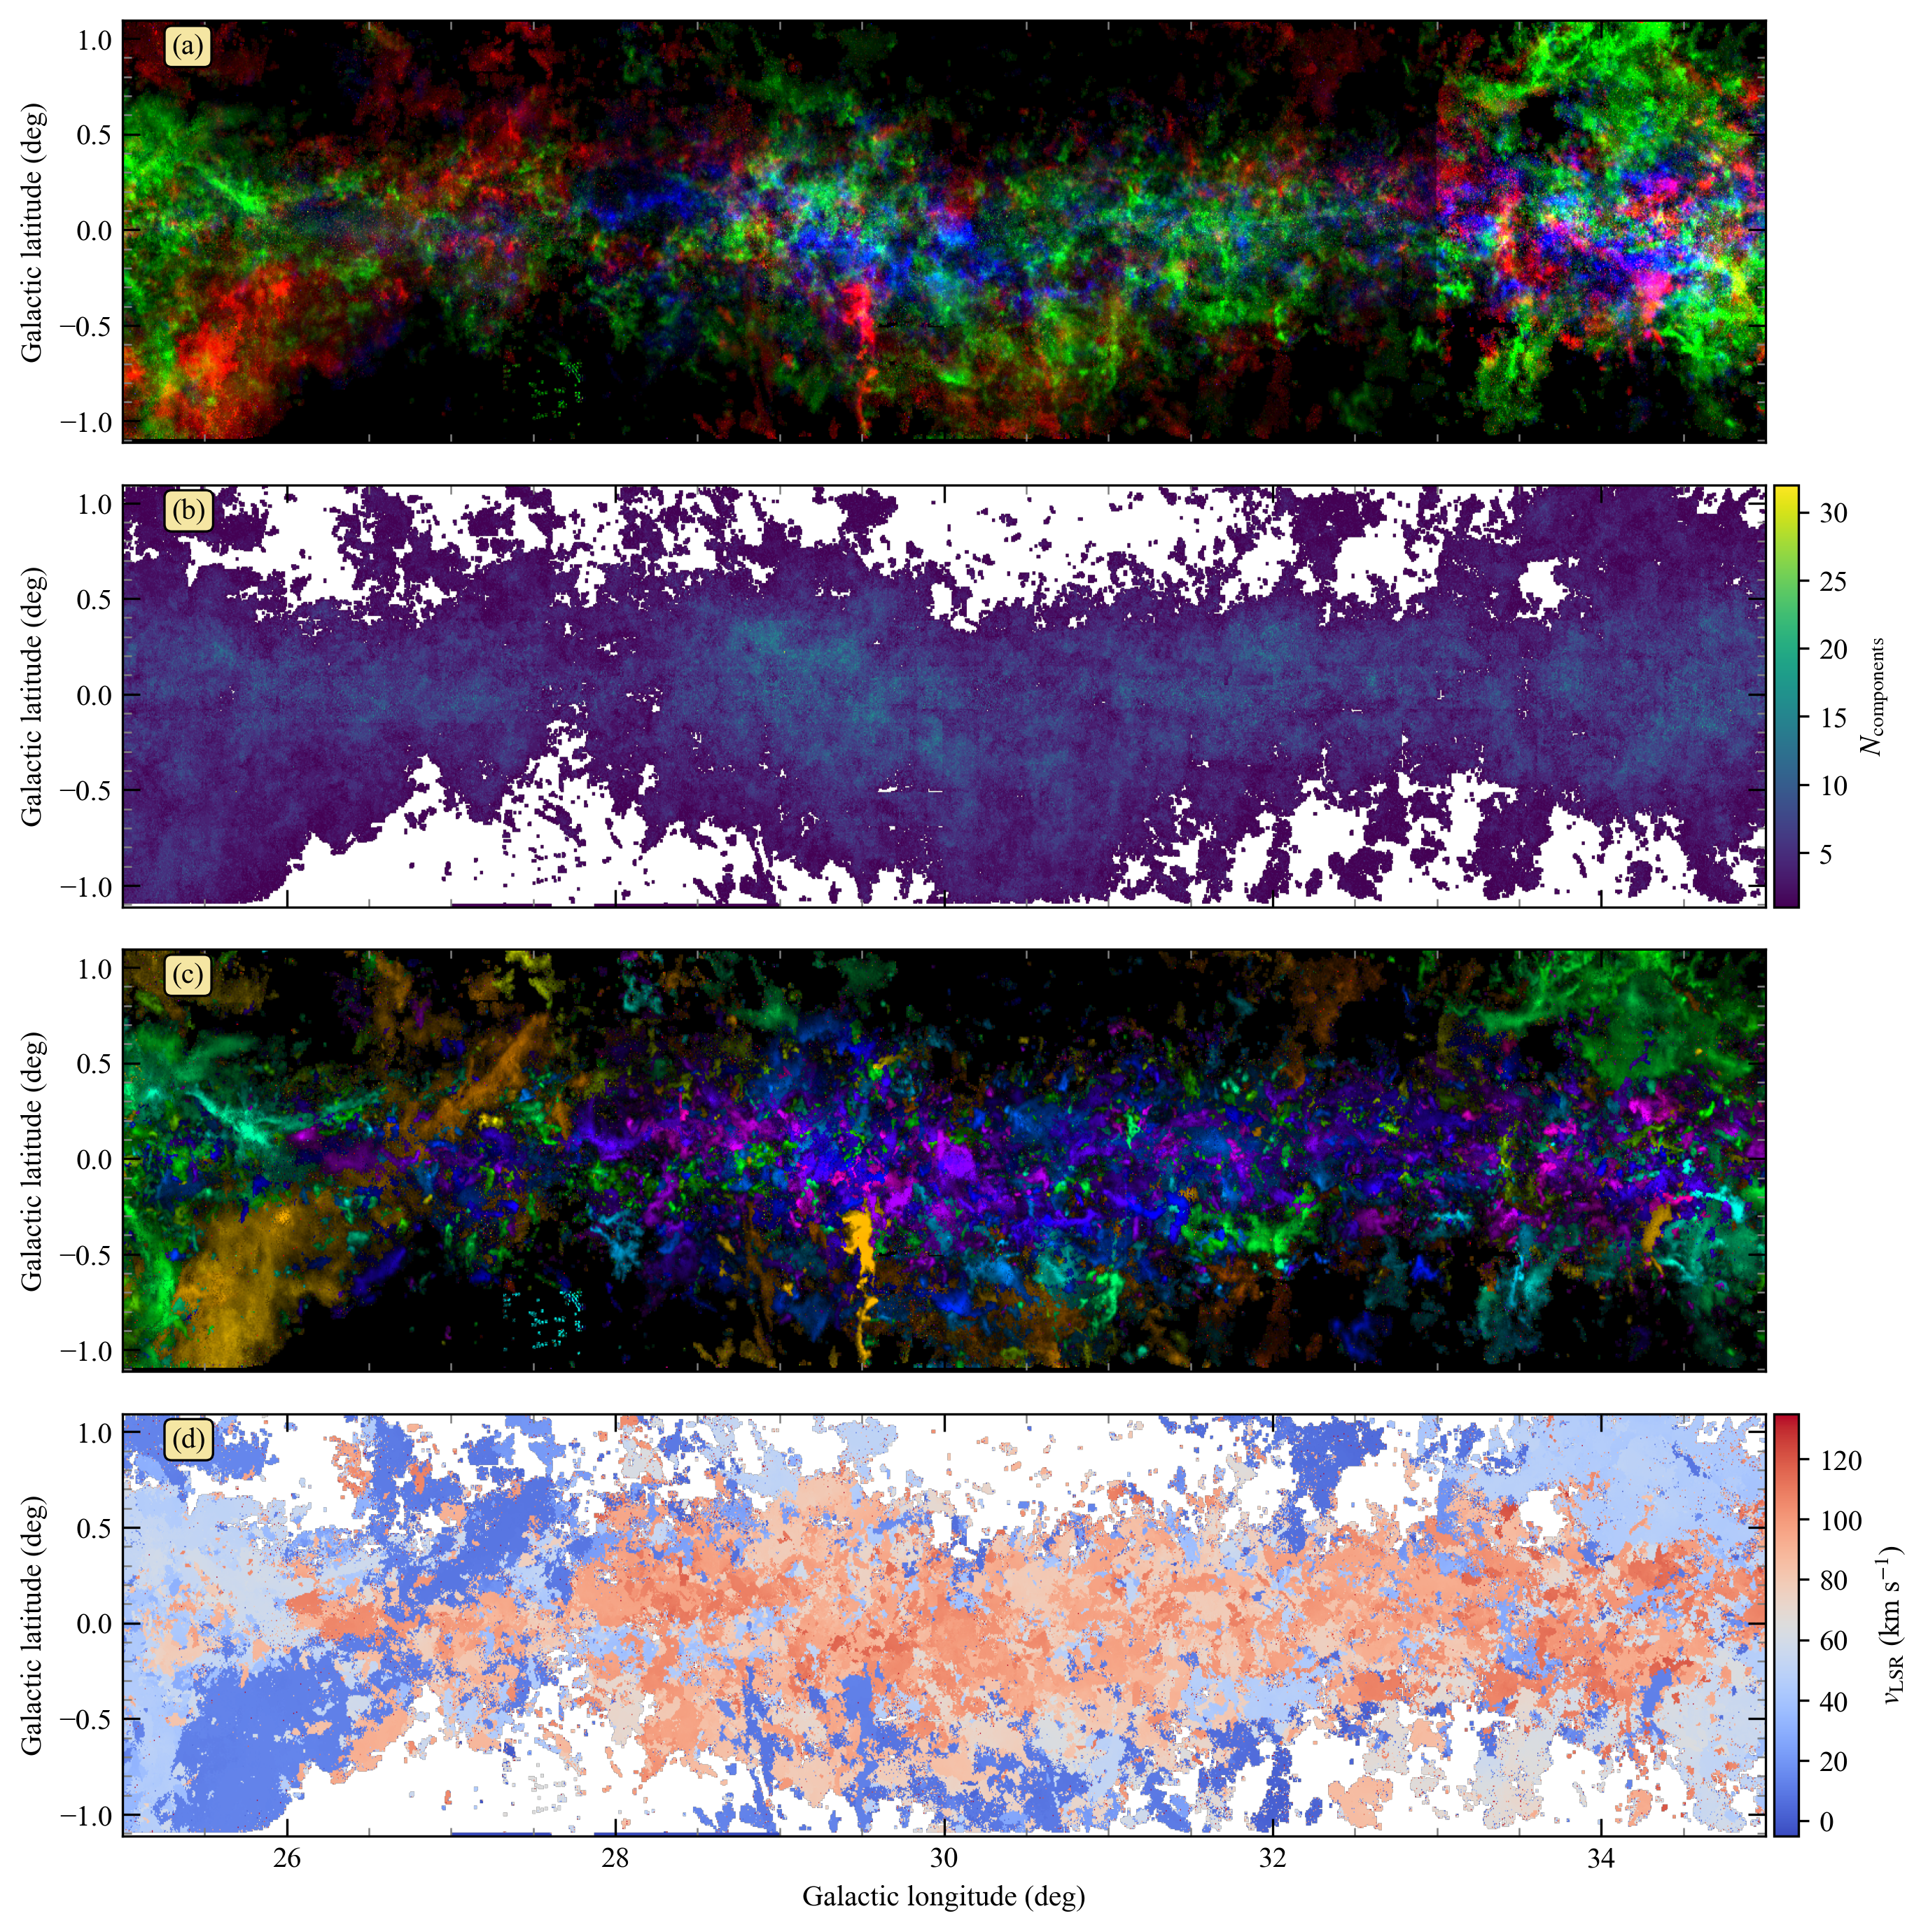
\includegraphics[width=\textwidth]{figures/img/grs-map-plot.png}
  \caption{%
    Four-panel decomposition strip of GRS tiles 26--34
    ($\ell \approx 25\degr$--$35\degr$).  \emph{(a)}~Velocity RGB
    composite: three velocity bins mapped to R, G, B from the decomposed
    Gaussians.  \emph{(b)}~Topological complexity: number of Gaussian
    components per pixel.  \emph{(c)}~Amplitude--velocity bivariate
    colormap: hue encodes centroid velocity, luminance encodes peak
    amplitude.  \emph{(d)}~Dominant velocity field: centroid velocity of
    the brightest component per pixel.
    \label{fig:grs_map}}
\end{figure*}

The two-point autocorrelation function $\xi(\theta)$ of each
derived field across the five-tile strip using FFT-based estimation, with
spatial-jackknife error bands ($4 \times 4$ block grid).  The structural
fields ($N_{\mathrm{comp}}$ and $I_{\mathrm{tot}}$) exhibit correlation
lengths of $\sim 0.3\degr$--$0.6\degr$, while the velocity fields
($\bar{v}$ and $\sigma_v$) decorrelate faster, consistent with the smaller
coherence scale of gas kinematics.  These scales match the angular sizes of
giant molecular cloud complexes in the inner Galaxy
\citep{RomanDuval2009,RomanDuval2010}, indicating that the decomposition
preserves spatial structure rather than imprinting spurious coherence.


% ============================================================================
% §4  PARAMETER SENSITIVITY
% ============================================================================
\section{Parameter sensitivity}\label{sec:beta}

The sole free parameter of \phspectra\ is $\beta$, which sets the minimum
persistence in units of noise (Equation~\ref{eq:threshold}).  Its
sensitivity on two independent benchmarks: the 350 synthetic spectra of
\S\ref{sec:synthetic}, where ground truth is known exactly, and a set of 52
hand-curated real GRS spectra scored against human-labeled decompositions.

On synthetic data the overall $F_1$ varies by only 0.040 across the full sweep
from $\beta = 2.0$ to 4.5 (\S\ref{sec:synthetic},
Figure~\ref{fig:synthetic_$f_1$}), peaking at $F_1$~$= 0.925$ at $\beta = 2.8$.
On the 52 real spectra, the optimal $\beta$ is 3.67, achieving
$F_1$~$= 0.576$ with precision $P = 0.43$ and recall $R = 0.89$.  The $F_1$
variation across the full sweep is 0.084 on real data.

The large gap between recall and precision on real data warrants
interpretation.  Recall $\approx 0.89$ means that \phspectra\ recovers
nearly 90\% of the components in the curated set.  Precision
$\approx 0.43$ means it consistently finds more components than the human
labeler marked.  Crucially, this precision deficit is \emph{stable across
$\beta$}: raising $\beta$ does not improve precision, because the extra
components are not noise artifacts (those would vanish at higher $\beta$).
They reflect genuine detections that fall outside the scope of the curated
labels --- faint or partially blended features that are easy to overlook
during manual inspection.  This interpretation is supported by the synthetic
benchmark, where precision and recall are both high ($F_1$~$= 0.925$),
confirming that \phspectra\ does not systematically hallucinate components.

\gausspyp\ requires the smoothing scales $\alpha_1$ and $\alpha_2$ to be
trained per survey (or per survey region) on synthetic spectra modeled after
the target data \citep{Lindner2015,Riener2019}.  Different regions of the
same survey can yield different optimal $\alpha$ values.  In contrast,
$\beta$ is survey-agnostic --- values in the range 2.8--3.7 work well
across both real and synthetic data --- and physically interpretable:
$\beta = 3.5$ means ``reject any peak whose persistence is less than a
$3.5\sigma$ fluctuation,'' a natural significance threshold.

The default $\beta = 3.5$ is adopted rather than $\beta = 2.8$ because the
accuracy cost is negligible ($F_1$ drops from 0.925 to 0.919 on synthetic
data, a difference of 0.006) while the computational benefit is
substantial: a lower $\beta$ admits more marginal candidates that must be
fitted by the Levenberg--Marquardt solver only to be rejected during
component validation, slowing the pipeline without improving the final
decomposition.

% ============================================================================
% §5  PERFORMANCE
% ============================================================================
\section{Performance}\label{sec:performance}

The wall-clock time for decomposing all 4200 GRS test-field
spectra (424 channels each) on a single core, with no parallelization for
either tool.  \phspectra\ uses the default $\beta = 3.5$ with its
C-accelerated Levenberg--Marquardt solver; \gausspyp\ is run in Docker with
Python~3.10 (required for compatibility with its dependencies).

Table~\ref{tab:timing} summarizes the results.  \phspectra\ is $2.0\times$
faster in total wall-clock time (746.4\,s vs.\ 1477.4\,s).  The two tools
have comparable median per-spectrum times (51.6\,ms vs.\ 40.4\,ms), but
their timing distributions differ sharply in the tails: \phspectra's P99 is
3.0\,s compared to \gausspyp's 8.4\,s, and these extreme outliers dominate
the aggregate timing.

Three algorithmic differences explain the speed advantage.  First,
\phspectra\ operates directly on the raw spectrum using persistence-based
peak detection, bypassing the smoothing sweep that \gausspyp\ performs at
each $\alpha$ scale.  Second, the C extension keeps per-call overhead low,
while \gausspyp's derivative-based approach can trigger costly iterative
refinement on complex spectra.  Third, \phspectra\ requires no separate
training step --- \gausspyp's $\alpha$ parameters must be trained per survey,
adding computational cost not reflected in the per-spectrum timing.

\begin{deluxetable}{lccc}
\tablecaption{Wall-clock timing benchmark on 4200 GRS spectra.
\label{tab:timing}}
\tablehead{
  \colhead{Metric} & \colhead{\phspectra} & \colhead{\gausspyp} &
  \colhead{Factor}
}
\startdata
Total time          & 746.4\,s   & 1477.4\,s  & $2.0\times$ \\
Mean per spectrum   & 177.7\,ms  & 350.5\,ms  & $2.0\times$ \\
Median per spectrum & 51.6\,ms   & 40.4\,ms   & ---         \\
P99 per spectrum    & 3.0\,s     & 8.4\,s     & $2.8\times$ \\
Components found    & 2.48       & 2.44       & ---         \\
\enddata
\end{deluxetable}



% ============================================================================
% §6  DISCUSSION
% ============================================================================
\section{Discussion}\label{sec:discussion}

Table~\ref{tab:comparison} places \phspectra\ in the context of three
established decomposition tools.  The distinguishing features are the use
of persistent homology for peak detection, the absence of training
requirements, and the intrinsic multi-scale nature of the persistence
filtration.  \gausspyp\ offers spatial coherence that \phspectra\ currently
lacks, while \rohsa\ provides full regularized optimization with built-in
coherence but requires manual tuning of regularization weights.

\paragraph{Scalability.}
Because each spectrum is decomposed independently, the algorithm is
trivially parallelizable.  A serverless pipeline has been deployed on
AWS Lambda that processes the full GRS ($\sim$2.3 million spectra) for
$\sim$\$40 in compute cost; the details of this infrastructure are beyond
the scope of this paper.

\paragraph{Limitations.}
Three limitations of the current approach should be noted; they are framed as
directions for future work.  First, \phspectra\ treats each spectrum
independently and does not enforce spatial coherence across neighboring
pixels.  \gausspyp\ uses a spatial refitting stage \citep[Section~3.3
of][]{Riener2019} that improves consistency across a data cube; a similar
post-processing step could be added to \phspectra.  Second, a single $\beta$
is used for all spectra in a survey.  While \S\ref{sec:beta} shows that
performance is robust to $\beta$ over a wide range, an adaptive $\beta$
that responds to local noise conditions could further improve performance
in surveys with spatially varying sensitivity.  Third, the algorithm assumes
Gaussian line profiles.  Non-Gaussian features such as self-absorption dips,
outflows, or Lorentzian wings are not modeled; extending the fitting stage
to support additional profile shapes is a natural next step.

\begin{deluxetable*}{lllll}
\tablecaption{Comparison of spectral line decomposition methods.
\label{tab:comparison}}
\tablehead{
  \colhead{Property} & \colhead{\phspectra} & \colhead{\gausspy} &
  \colhead{\gausspyp} & \colhead{\rohsa}
}
\startdata
Peak detection    & Persistent homology   & Derivative spectroscopy & Derivative spectroscopy & Regularized optimization \\
Free parameters   & $\beta$ only          & $\alpha_1$, $\alpha_2$  & $\alpha_1$, $\alpha_2$, SNR thresholds & $\lambda$ weights \\
Training          & None (default works)  & Required (synthetic)    & Required (synthetic)    & Manual tuning \\
Spatial coherence & No                    & No                      & Yes                     & Yes \\
Model selection   & AICc                  & BIC                     & BIC + heuristics        & Regularization \\
Multi-scale       & Intrinsic             & Per-$\alpha$ scale      & Per-$\alpha$ scale      & Regularized \\
Speed (GRS)       & 178\,ms/spectrum      & ---                     & 351\,ms/spectrum        & --- \\
\enddata
\end{deluxetable*}


% ============================================================================
% §7  SUMMARY
% ============================================================================
\section{Summary}\label{sec:summary}

\phspectra\ is presented as a new tool for automated Gaussian
decomposition of spectral lines based on 0-dimensional persistent homology.
The key results are:

\begin{enumerate}
  \item \textbf{First application of persistent homology to spectral line
    decomposition.}  The algorithm detects peaks by tracking the birth and
    death of connected components in the signal's upper-level sets as a
    threshold descends from the global maximum, ranking features by their
    topological persistence without smoothing or differentiation.

  \item \textbf{Single parameter, no training.}  The sole free parameter is
    $\beta = 3.5$ (the persistence threshold in units of noise), which
    requires no survey-specific training and is physically interpretable as
    a significance threshold.

  \item \textbf{High accuracy on synthetic data.}  On a benchmark of 350
    spectra spanning seven difficulty categories, \phspectra\ achieves an
    overall $F_1$~$= 0.925$ at the optimal $\beta = 2.8$, with performance
    varying by only 0.040 across $\beta \in [2.0, 4.5]$.

  \item \textbf{Competitive on real data.}  Compared with \gausspyp\ on
    4200 real ${}^{13}$CO spectra from the GRS, \phspectra\ achieves lower
    residual RMS on 62\% of head-to-head comparisons.  Cases where
    \gausspyp\ achieves lower RMS are associated with high component counts
    (8.2 on average for RMS~$> 0.2$~K vs.\ \phspectra's 1.6), consistent
    with overfitting.

  \item \textbf{Faster execution, better tail behavior.}  \phspectra\ is
    $2.0\times$ faster in total wall-clock time on the same 4200 spectra,
    with a P99 latency of 3.0\,s compared to 8.4\,s for \gausspyp.

  \item \textbf{Open-source.}  The software, documentation, and benchmark
    scripts are publicly available at
    \url{https://github.com/caverac/phspectra}.
\end{enumerate}

Future work will focus on adding spatial coherence for cube-level
decomposition, applying \phspectra\ to HI 21\,cm surveys, and producing a
full GRS decomposition catalog.

The central result is that persistent homology enables a survey-ready,
parameter-light decomposition that matches trained methods while eliminating
their tuning burden, making large-scale spectral analysis faster, more
reproducible, and easier to deploy.

% ============================================================================
% ACKNOWLEDGMENTS
% ============================================================================
% TODO: acknowledgments

% ============================================================================
% APPENDIX
% ============================================================================
\appendix

\section{Implementation Details}\label{app:implementation}

% ---------------------------------------------------------------------------
% A.1  Union-find pseudocode
% ---------------------------------------------------------------------------
\subsection{Union-find persistence algorithm}\label{app:unionfind}

Algorithm~\ref{alg:persistence} gives the pseudocode for the 0-dimensional
persistence peak detection used in \phspectra.  The algorithm processes
samples in decreasing order of function value, maintaining a union-find
structure to track connected components.

\begin{figure}[t!]
\centering
\fbox{\parbox{0.92\columnwidth}{%
\small
\textbf{Algorithm 1:} 0-dimensional persistence peak detection\\[4pt]
\textbf{Input:} Signal $f[0..n{-}1]$, threshold $\pmin$\\
\textbf{Output:} List of peaks with persistence $> \pmin$\\[4pt]
1.\quad $\mathrm{order} \gets \mathrm{argsort}(-f)$
  \hfill\textit{// decreasing value}\\
2.\quad Initialize union-find on $\{0, \ldots, n{-}1\}$\\
3.\quad $\mathrm{visited}[i] \gets \mathrm{false}$ for all $i$;
  \quad $\mathrm{peaks} \gets \{\}$\\
4.\quad \textbf{for} $\mathrm{idx}$ \textbf{in} $\mathrm{order}$ \textbf{do}\\
5.\quad\quad $\mathrm{visited}[\mathrm{idx}] \gets \mathrm{true}$\\
6.\quad\quad \textbf{for} $\mathrm{nbr} \in \{\mathrm{idx}{-}1,\;
  \mathrm{idx}{+}1\}$ \textbf{do}\\
7.\quad\quad\quad \textbf{if} $0 \leq \mathrm{nbr} < n$ \textbf{and}
  $\mathrm{visited}[\mathrm{nbr}]$ \textbf{then}\\
8.\quad\quad\quad\quad $r_1 \gets \mathrm{Find}(\mathrm{idx})$;\;
  $r_2 \gets \mathrm{Find}(\mathrm{nbr})$\\
9.\quad\quad\quad\quad \textbf{if} $r_1 \neq r_2$ \textbf{then}\\
10.\quad\quad\quad\quad\quad Identify younger component (lower peak)\\
11.\quad\quad\quad\quad\quad $\pi \gets f[\mathrm{younger}] -
  f[\mathrm{idx}]$\\
12.\quad\quad\quad\quad\quad \textbf{if} $\pi > \pmin$ \textbf{then}
  record peak\\
13.\quad\quad\quad\quad\quad $\mathrm{Union}(r_1, r_2)$\\
14.\quad Record global maximum (persistence $= f[\mathrm{order}[0]]$)\\
15.\quad \textbf{return} peaks sorted by persistence (descending)%
}}
\caption{Pseudocode for the union-find persistence peak detection algorithm
used in \phspectra.  The algorithm processes samples in decreasing order of
function value, merging connected components via union-find and recording
birth--death pairs.\label{alg:persistence}}
\end{figure}

% ---------------------------------------------------------------------------
% A.2  Noise estimation
% ---------------------------------------------------------------------------
\subsection{Noise estimation algorithm}\label{app:noise}

% TODO: Detailed pseudocode for the signal-masked RMS estimation:
% 1. Find runs of consecutive positive channels
% 2. Mask runs > 2 channels wide (with pad=2 on each side)
% 3. MAD from negative unmasked channels
% 4. Clip channels > 5*sigma_MAD
% 5. Final RMS from surviving channels
% 6. Fallback to simple MAD if < 5 channels survive

% ---------------------------------------------------------------------------
% A.3  Software availability
% ---------------------------------------------------------------------------
\subsection{Software availability}\label{app:software}

\phspectra\ is open-source software written in Python.  The source code,
documentation, and benchmark scripts are available at
\url{https://github.com/caverac/phspectra}.  The package depends on
NumPy \citep{Harris2020} and SciPy \citep{Virtanen2020}.

% ============================================================================
\bibliography{ms}
\bibliographystyle{aasjournal}

\end{document}
